%-----------------------------------------------------------------------------%
\chapter{LANDASAN TEORI}
%-----------------------------------------------------------------------------%
\vspace{4.5pt}
Pada bab ini menjelaskan beberapa teori dan jurnal yang berhubungan dengan permasalahan penelitian yang digunakan pada proses penelitian.
\section{Tinjauan Pustaka}
Pembahasan mengenai teori-teori tersebut dijelaskan sebagai berikut.
\subsection{Monolit}
Monolit yaitu suatu cara untuk melakukan penyebaran. Ketika semua fungsi dalam sistem harus disebarkan secara bersama-sama, maka itu merupakan sebuah monolit \cite{74C}. Monolit merupakan sebuah aplikasi perangkat lunak dimana setiap modulnya tidak bisa dieksekusi secara independen. Hal ini membuat monolit sulit digunakan pada sistem terdistribusi tanpa bantuan penggunaan \textit{frameworks} atau solusi \textit{ad hoc} seperti Objek Jaringan, \textit{RMI} atau \textit{CORBA} \cite{0BD}.

Penggunaan pada bahasa pemrograman seperti \textit{Java},\textit{C/C++}, dan \textit{Python} pada pengembangan aplikasi di sisi \textit{server}, memiliki kemampuan dalam melakukan abstraksi untuk memecah kompleksitas program menjadi berupa modul. Namun, bahasa pemrograman ini dirancang untuk membuat \textit{artefacts} monolit. Dimana abstraksi ini tergantung pada penggunaan berbagi sumber data pada komputer yang sama (memori, database, file) \cite{0BD}.


Terdapat 3 jenis monolit \cite{74C}:
\begin{enumerate}[leftmargin=1.3cm]
\item \textit{Single Process Monolith}\\
Dimana sebuah kode disebarkan dengan satu proses. Setiap kode bisa berada di banyak \textit{instances} serta tempat penyimpanan dan mendapatkan data disimpan pada suatu database yang sama. Variasi lainnya yaitu modular monolit dimana setiap kode bisa bekerja secara independen tetapi perlu dijadikan satu kesatuan ketika ingin dilakukan \textit{deployment}.
\item \textit{Distributed Monolith}\\
Monolit terdistribusi adalah sistem yang terdiri dari beberapa layanan, tetapi untuk apa pun alasannya seluruh sistem harus disebarkan bersama-sama. Sebuah monolit terdistribusi bisa memiliki kesamaan dengan \textit{service-oriented architecture (SOA)}.

Monolit terdistribusi biasanya muncul  di kondisi dimana tidak cukup fokus pada konsep \textit{information hiding} dan kohesi dari fungsi bisnis. Akibatnya terbentuklah arsitektur yang memiliki kopel yang tinggi, dimana bisa perubahan menyebabkan kerusakan pada bagian sistem lain.
\item \textit{Sistem Black-Box Pihak Ketiga}\\
Aplikasi pihak ketiga merupakan sebuah monolit, misalkan sistem penggajian, sistem CRM, dan sistem SDM. Faktor umum yang terjadi yaitu aplikasi ini dibuat dan dikelola oleh orang lain dimana pengembang belum tentu memiliki kemampuan untuk mengubah kode seperti \textit{Software-as-a-Service(SaaS)}.
\end{enumerate}

Keuntungan dari Monolit \cite{ECD,1C7}:
\begin{enumerate}[leftmargin=1.3cm]
\item Sederhana dalam melakukan pengembangan karena \textit{Integrated Development Environment (IDE)} dan peralatan pengembang berfokus pada membuat satu aplikasi
\item Mudah untuk melakukan perubahan secara radikal di aplikasi. Perubahan ini bisa dari kode hingga skema database serta proses \textit{deployment}.
\item Pengujian dilakukan pada satu aplikasi, pengembang dapat membuat pengujian dari awal hingga akhir dengan lebih mudah dan terintegrasi
\item Deployment dilakukan pada satu aplikasi, pengembang hanya menyalin aplikasi dari komputer ke komputer yang lain. Dengan ini aplikasi relatif mudah dilakukan konfigurasi dan mudah diperbanyak jumlah aplikasi.
\end{enumerate}

Tantangan dari monolit \cite{ECD,1C7}:
\begin{enumerate}[leftmargin=1.3cm]
	\item Sulit dikembangkan secara berkelanjutan, karena semakin banyak orang yang bekerja pada aplikasi yang sama. Akibatnya setiap pengembang memiliki kepentingan masing-masing dalam mengelola kode yang sama dan membuat pengambilan keputusan sulit serta tidak fleksibel
	\item Memiliki reliabilitas yang rendah, karena kesalahan pada salah satu module aplikasi bisa menyebabkan kegagalan secara keseluruhan aplikasi. Akibatnya aplikasi tidak dapat digunakan oleh pengguna dan harus dilakukan deployment kembali.
	\item Tidak mudah untuk melakukan skalabilitas,setiap modul aplikasi memiliki kebutuhan sumber daya yang berbeda seperti ada module penyediaan data yang membutuhkan banyak memori sedangkan modul pemprosesan gambar membutuhkan banyak CPU, karena module ini berada pada aplikasi yang sama akibatnya pengembang harus melakukan pengorbanan pada salah satu sisi sumber daya.
	\item Terkunci pada teknologi jadul, pengembang terkunci pada teknologi awal yang digunakan untuk membangun aplikasi. Pengembang juga kesulitan ketika ingin mengadopsi teknologi baru pada aplikasi karena sangat berisiko dan sangat mahal untuk menulis kembali seluruh aplikasi antar teknologi.\\
\end{enumerate}	

\subsection{\textit{Microservice}}
\textit{Microservice} adalah beberapa \textit{service} yang bisa di deploy secara independen yang dimodelkan berdasarkan bisnis domain. \textit{Service} ini berkomunikasi satu sama lain melalui jaringan komputer dan bisa dibangun dengan berbagai macam teknologi. \textit{Microservice} adalah salah tipe dari \textit{service oriented architecture (SOA)} meskipun ada perbedaan dalam membuat batasan antara \textit{service} dan \textit{deployment} secara independen \cite{1C7}.

\textit{Service} adalah komponen perangkat lunak yang memiliki kegunaannya secara khusus dimana komponen ini bisa berdiri sendiri dan secara independen dilakukan proses deployment. Service memiliki \textit{API (Application Programming Interface)} yang memberikan akses kepada \textit{client} untuk melakukan operasi. Terdapat 2 tipe operasi yaitu perintah dan kueri.
\textit{API} terdiri dari perintah, kueri dan \textit{event}. Perintah dapat berupa \textit{buatPesanan()} yang melakukan aksi dan memperbarui data. Kueri dapat berupa \textit{cariPesananBerdasarkanID()} yang digunakan untuk mengambil data. \textit{Service} juga dapat membuat suatu \textit{event} seperti \textit{PesananSudahDibuat} dimana \textit{event} ini akan dikonsumsi oleh \textit{client}-nya / \textit{subscriber} \cite{1C7}.

\textit{Service API} akan mengenkapsulasi internal implementasinya, sehingga pengembang aplikasi tidak bisa menuliskan kode yang melewati \textit{API}. Akibatnya arsitektur \textit{microservice} dapat mewajibkan modularitas di aplikasi.  Setiap \textit{service} di arsitektur \textit{microservice} memiliki masing-masing arsitektur sendiri dan dimungkinkan dengan teknologi yang berbeda. Tetapi kebanyakan \textit{service} memiliki arsitektur heksagonal. Dimana \textit{API} akan diimplementasi melalui adapter yang berinteraksi dengan logika bisnis \cite{BC4}

Ciri Khusus \textit{Microservice} \cite{ECD,BC4,1C7}:	
\begin{enumerate}[leftmargin=1.3cm]
	\item Kecil dan berfokus pada satu hal dengan baik\\
	\textit{Service} yang dibuat memiliki \textit{encapsulation} dengan pembuatan \textit{service} dimodelkan di sekitar Domain Bisnis, tujuannya agar ketika terjadi perubahan antar \textit{service} bisa dilakukan dengan lebih mudah dan tidak berdampak pada \textit{service} lain. Oleh karena itu \textit{service} yang dibuat seminimal mungkin untuk tidak berhubungan dengan \textit{service} lain. 
	\item Otonomi / Bisa berdiri sendiri\\
	\textit{Microservice} memiliki \textit{service} yang terisolasi dimana bisa memiliki sistem operasi hingga komputer yang berbeda. Dengan ini sistem terdistribusi lebih sederhana dan nilai kopel yang rendah. Semua komunikasi antar service dilakukan melalui jaringan sehingga \textit{service} harus memiliki kemampuan di\textit{deploy} sendiri tanpa harus mempengaruhi \textit{service} lain.
	\item Data yang dikelola masing-masing \textit{service}\\
	\textit{Service} yang membutuhkan data diluar domainnya harus berkomunikasi melalui \textit{API(application programming interface)}, dengan ini setiap \textit{service} memiliki tanggung jawab terhadap datanya masing-masing sehingga data tersebut hanya bisa diubah oleh \textit{service} itu sendiri. Setiap \textit{service} memiliki data yang pribadi dan data yang bisa dibagikan kepada \textit{service} lain
\end{enumerate}	

Keuntungan dari \textit{Microservice}  \cite{ECD,BC4,1C7}:
\begin{enumerate}[leftmargin=1.3cm]
	\item Memudahkan pengembangan aplikasi kompleks dan flexibel\\
	\textit{Service} berukuran kecil sehingga mudah dikelola, perubahan pada satu \textit{service} bisa diterapkan secara independen dari service lainnya. Bila terjadi kegagalan di satu \textit{service} tidak berdampak besar pada \textit{service} lainnya karena \textit{service} masing-masing terisolasi selain itu proses pemulihan bisa dilakukan dengan mudah dan cepat.
	\item Bisa dilakukan skaling secara independen\\ 
	Setiap \textit{service} memiliki fungsi yang berfokus pada satu hal,  dimana setiap \textit{service} bisa memiliki kebutuhan sumber daya berbeda. Penggunaan sumber daya ini bisa dikelola dengan mudah dan cepat karena setiap service dapat di\textit{deploy} dengan jumlah \textit{service} yang berbeda.
	\item Mudah melakukan percobaan dan penggunaan teknologi baru\\
	Arsitektur \textit{microservice} mengeliminasi komitmen penggunaan secara lama pada suatu teknologi. Dengan ini pengembang dapat memilih berbagai teknologi dalam membangun \textit{service} serta \textit{service} yang kecil dan berfokus lebih mudah untuk dilakukan migrasi antara teknologi yang berbeda. 
\end{enumerate}	

Tantangan dari \textit{Microservice}  \cite{ECD,BC4,1C7}:
\begin{enumerate}[leftmargin=1.3cm]
	\item Menemukan \textit{service} yang tepat itu sulit\\
	Salah satu tantang terbesar dari membuat \textit{microservice} yaitu tidak adanya cara yang pasti bagaimana untuk melakukan dekomposisi dengan baik. Dimana \textit{service} yang didekomposisi dengan tepat tidak mudah ditemukan dan bila dilakukan dengan tidak benar dapat sebaliknya membuat \textit{distributed monolith}. 
	\item Memiliki kompleksitas karena merupakan suatu terdistribusi\\
	Setiap \textit{service} untuk berkomunikasi antar \textit{service} memiliki tantangan masing-masing seperti latensi, konsistensi data, dan kondisi ketika beberapa \textit{service} mengalami kegagalan. \textit{Microservice} juga meningkatkan kompleksitas operasional oleh karena itu untuk melakukan \textit{deployment} sebaiknya menggunakan proses otomatisasi.
	\item \textit{Deployment} yang melibatkan beberapa service\\
	Untuk melakukan \textit{deployment} ini dibutuhkan koordinasi antara tim pengembang \textit{servic} ketika menambahkan atau mengubah fitur yang berdampak pada beberapa \textit{service} maka dari itu harus dibuat perencanaan \textit{deployment} berdasarkan ketergantungan antar \textit{service}.
\end{enumerate}	

Pola Arsitektur \textit{Microservice}  \cite{1C7}:
\begin{center}
	\includegraphics[width=12cm]{img/PolaMicroservice.png}
	\captionof{figure}{
	Pola dalam menyelesaikan masalah di arsitektur \textit{Microservice} \cite{1C7} }
	\label{fig:msa}
\end{center}
\begin{enumerate}[leftmargin=1.3cm]
	\item \textit{Application patterns}\\
	Permasalahan yang harus diselesaikan oleh pengembang aplikasi, yaitu bagaimana cara dekomposisi sistem menjadi beberapa service. Terdapat beberapa Strategi yang dapat dilakukan seperti berdasarkan sub-domain dan berdasarkan proses bisnis. Service mengelola datanya masing-masing namun ini menyebabkan permasalahan tersendiri karena bisa terjadi data yang tidak konsisten antara service. Pendekatan biasa seperti 2PC tidak cocok pada aplikasi modern sehingga konsistensi data dicapai melalui SAGA.
	
	Perbedaan penyimpanan data membuat kueri harus menggabungkan data yang dimiliki oleh beberapa service yang terlibat karena data hanya bisa diakses melalui API. Terkadang bisa digunakan komposisi API dimana memanggil API service satu dengan yang lain atau dengan Command Query Responsibility Seqgregation(CQRS) yaitu ketika setiap service memiliki replika data dari service yang dibutuhkan.

	Pengujian pada service mudah dilakukan karena memiliki lingkup yang kecil dan terpusat namun untuk menguji beberapa service tidak mudah, karena banyaknya proses yang harus dilakukan. Sehingga diperlukan proses otomatisasi proses pengujian. Ada beberapa pola yang dapat digunakan untuk pengujian di microservice yaitu test dilakukan pada client/konsumen, test pencocokan pada client/konsume, dan pengujian secara terisolasi.  

	\item \textit{Application infrastructure} \\
	Permasalah infrastruktur yang memiliki pengaruh pada proses pengembangan aplikasi. Aplikasi yang dibangun dengan microservice merupakan sistem terdistribusi. Sehingga komunikasi antar proses adalah bagian yang penting dapat arsitektur microservice. Diperlukan variasi arsitektur dan keputusan desain tentang bagaimana service berkomunikasi satu dengan yang lain. 

	Pola komunikasi dikelompokan menjadi 5 grup yaitu gaya komunikasi, dicovery, reliabilitas, Transactional Messaging, API Eksternal. Terdapat 3 gaya komunikasi yaitu Messaging dimana komunikasi dapat dilakukan secara asynchronous, Domain-Specific dimana komunikasi harus melalui protokol tertentu seperti Email, dan Remote Procedure Invocation dimana komunikasi dilakukan secara asynchronous.
	
	Cara Messaging memiliki kelemahan karena transaksi terdistribusi tidak cocok digunakan pada aplikasi modern untuk mengatasi ini ada 2 pendekatan yaitu polling publisher dimana menggunakan tabel OUTBOX untuk menyimpan message sementara dan Log Tailing dimana melihat transaksi terakhir dari message.

	Ketika service sedang berkomunikasi dan waktu menunggu jawaban dari service lain melebihi batas yang ditentukan maka bisa terjadi kemungkinan service tersebut mengalami kegagalan. Pola Circuit Breaker dapat diterapkan bila terjadi hal seperti ini tujuannya agar service tidak berkomunikasi pada service yang gagal.

	Pada arsitektur microservice untuk proses authentikasi pengguna umumnya dilakukan oleh API Gateway. Dimana API Gateway melanjutkan informasi ke service yang bertanggung jawab mengenai authentikasi, solusi umumnya yaitu menggunakan Access Token seperti JWT(JSON Web Token).
	\item \textit{Infrastructure patterns}\\
	Permasalahan infrastruktur yang muncul diluar dari pengembangan aplikasi. Infrastruktur menangani proses deployment, discovery, dan External API. 
	Discovery adalah bagaimana service bisa ditemukan agar bisa berkomunikasi, terdapat beberapa pendekatan yang bisa dilakukan seperti service ditemukan dari client atau dari server dan proses registrasi bisa dilakukan secara sendiri atau melalui pihak ke-3.

	Eksternal API adalah bagaimana aplikasi pengguna berinteraksi dengan service.
	Ada 2 cara untuk aplikasi berinteraksi yaitu API Gateway dan Backend for Frontend. Proses Deployment microservice memiliki proses yang kompleks karena service yang dikelola bisa berjumlah 10 hingga ratusan service, sehingga diperlukan proses otomatisasi yang bisa mengelola service dan proses skaling bisa diatur berdasarkan kebutuhan. Cara melakukan deployment bisa dengan container, virtual machine, serverles, atau menggunakan platform deployment \\	
\end{enumerate}	

\subsection{\textit{Enterprise Resource Planning}}
\textit{Enterprise Resource Planning} (ERP) adalah suatu sistem perangkat lunak yang memungkinkan perusahaan untuk mengotomatisasikan dan mengintegrasikan proses bisnisnya dengan komputerisasi. Dengan ini setiap informasi yang diperlukan di proses bisnis dapat dibagikan dan digunakan disemua bagian perusahaan dengan alur terstruktur. Sistem ERP dapat mengeliminasi duplikasi data dan memberikan integrasi data. Sistem ERP memiliki database dimana semua transaksi bisnis dapat direkam, diproses, dipantau dan dilaporkan. Tujuannya agar proses bisnis bisa dilakukan dengan lebih cepat, murah, dan transparan \cite{D94}.

Sistem ERP dapat memberikan dukungan untuk proses bisnis perusahaan melalui modul yang terpisah. Setiap modul adalah aplikasi perangkat lunak yang dibangun khusus untuk setiap operasi bisnis. Umumnya modul yang ditemukan pada ERP yaitu Modul Produksi, Modul Manajemen Rantai Pasokan, Modul Keuangan, Modul Penjualan \& Pemasaran, Modul Sumber Daya Manusia, dan modul pelengkap lainnya seperti \textit{e-commerce} \cite{D94}.

Arsitektur ERP \cite{D94}: 
\begin{enumerate}[leftmargin=1.3cm]
	\item \textit{The Tiered}\\
	Arsitektur \textit{tiered} umumnya dirancang dalam bentuk lapisan yang didasarkan dari model \textit{client-server} atau bisa disebut \textit{N-Tier}. Dalam arsitektur ini setiap komponen ERP disusun kedalam masing lapisan seperti lapisan \textit{user interface}, lapisan aplikasi dan lapisan \textit{database} / penyimpanan data.
	\item \textit{Web-based}\\
	Arsitektur \textit{Web-based} mengadopsi teknologi berorientasi objek web dimana pengguna yang ingin menggunakan sistem ERP bisa mengakses melalui \textit{browser} dan internet. \textit{Object-oriented technology} diimplementasi untuk mencampur data dan fungsi yang tersedia di berbagai web \textit{service}.
	\item \textit{Service Oriented}\\
	\textit{SOA(Service Oriented Architecture)} adalah sistem yang dimana terdapat fungsi  modular yang berkomunikasi melalui jaringan. Satu atau lebih \textit{service} bisa berkordinasi dalam suatu aktivitas fungsi bisnis. 
	\item \textit{Cloud}\\
	\textit{Cloud} dapat memberikan solusi bagi organisasi ketika mengadopsi sistem ERP pada kegiatan bisnisnya. Sistem ERP dengan arsitektur \textit{cloud} bisa dikategorikan sebagai tipe \textit{SaaS(Software as a Service)}. Organisasi akan membayar pihak ke tiga setiap periode berdasarkan modul yang digunakannya.\\ 
\end{enumerate}

\subsection{Analisis Kode}
Analisis Kode adalah suatu proses mengekstraksi informasi mengenai suatu program dari kode atau artifak. Proses ini bisa dilakukan secara manual yaitu dengan melihat kode program atau bahasa mesin namun kompleksitas program yang tinggi membuat proses secara manual sangat sulit dan tidak efektif. Sehingga diperlukan alat otomatisasi yang dapat membantu proses analisis kode. Alat ini dapat memberikan informasi kepada pengembang mengenai program yang dianalisis \cite{208}. 

Anatomi Analisis Kode \cite{208}:
\begin{enumerate}[leftmargin=1.3cm]
	\item Ekstraksi Data\\
	Proses ini adalah proses pertama kali dilakukan sebelum melakukan analisis kode, data yang diekstrasi berasal dari kode program. Umumnya dilakukan dengan \textit{syntatic analyzer} atau \textit{parser}. Proses \textit{Parser} ini mengkonversi urutan karakter menjadi suatu kata-kata dan mengekstraksi nilai semantik sebenarnya. Tujuannya agar memudahkan proses analisis/transformasi dan penambahan data lainnya.
	\item Representasi Informasi\\
	Proses yang merepresentasikan informasi kode menjadi bentuk yang lebih abstrak. Tujuan dari fase ini untuk membentuk beberapa bagian kode agar terhubung pada analisis secara otomatis. Representasi ini kebanyakan berupa graph seperti \textit{Abstract Syntax Trees (AST)}, \textit{Control Flow Graphs (CFG)}, dan \textit{Call Graph}.
	\item Eksplorasi Pengetahuan\\
	Setelah informasi direpresentasikan, informasi dibuat menjadi suatu kesimpulan. Kesimpulan bisa dibuat secara kuantitatif atau kualitatif, proses visualisasi penting dalam proses eksplorasi pengetahuan kode program.
\end{enumerate}

Strategi Analisis Kode \cite{208}:
\begin{enumerate}[leftmargin=1.3cm]
	\item Statik vs Dinamis\\
	Analisis secara statik menganalisis program tanpa dieksekusi untuk mendapatkan semua informasi yang kemungkinan akan dieksekusi. Sedangkan secara Dinamis, program mengumpulkan informasi yang dieksekusi dengan nilai yang diberikan. Beberapa teknik analisis menggabungkan kedua pendekatan ini.
	\item \textit{Sound vs Unsound}\\
	\textit{Sound} yaitu analisis yang bisa menjamin secara keseluruhan dan kebenaran eksekusi program. Sedangkan \textit{Unsound} tidak bisa secara keseluruhan menjaminkan kebenaran hasil analisis program. Namun dalam banyak kasus analisis \textit{Unsound} memiliki hasil yang benar selain itu memiliki kelebihan yaitu mudah diimplementasi dan efisien.
	\item \textit{Flow sensitive vs Flow insensitive}\\
	\textit{Flow sensitive} memperhatikan dan menyimpan urutan proses eksekusi sedangkan \textit{Flow insensitive} tidak memperhatikan urutan proses eksekusi sehingga tidak memiliki informasi ketergantungan pada suatu proses dan hanya dapat menyatakan proses tersebut ada.
	\item \textit{Context sensitive vs Context insensitive}\\
	\textit{Context in-sensitive} hanya menghasilkan satu hasil yang berhubungan dalam semua konteks. Sedangkan \textit{context sensitive} memiliki hasil berbeda ketika konteks berbeda. Pendekatan ini bertujuan untuk menganalisis proses pembuatan analisis umumnya tanpa adanya informasi mengenai konteks yang akan digunakan. \textit{Context sensitive} penting untuk menganalisis program modern dimana terdapat suatu abstraksi.
\end{enumerate}

Tantangan Kode Analisis \cite{208}:
\begin{enumerate}[leftmargin=1.3cm]
	\item Perbedaan bahasa kode program\\
	Banyak peningkatan dan perubahan pada bahasa pemrograman seperti \textit{dynamic class loading} dan \textit{reflection}. Konsep ini juga terdapat pada proses pengubahan tipe data, \textit{pointer}, \textit{Anonymous types} yang membuat proses \textit{parser} sulit. Fitur pada pemrograman ini meningkatkan fleksibilitas ketika program berjalan dan membutuhkan analisis secara dinamik yang lebih kuat.
	\item \textit{Multi-Language}\\
	Banyak aplikasi yang dibuat sekarang dibangun dengan berbagai bahasa pemrograman. Dimana sekarang perlengkapan pembuatan aplikasi masih belum bisa menganalisis secara keseluruhan pada aplikasi yang menggunakan banyak bahasa pemrograman. Seperti aplikasi berbasis web yang memiliki \textit{HTML}, \textit{ASP}, \textit{Java} dan lainnya.
	\item Analisis secara \textit{Real-Time}\\
	Analisis ini dapat memberikan keuntungan bagi pengembang karena memberikan informasi tambahan selama pengembang membuat aplikasi seperti \textit{code coverage} dan analisis kebocoran memori. Proses analisis juga kerap kali membutuhkan penggunaan sumber daya komputasi yang tinggi dan memori yang banyak.\\
\end{enumerate}

\subsection{\textit{Clustering}}
\textit{Clustering} yaitu suatu proses untuk melakukan pengelompok atau klasifikasi objek. Objek bisa ditentukan dari pengukuran atau berdasarkan hubungan antar objek lainnya. Tujuan dari clustering yaitu untuk  menemukan struktur data yang valid. Cluster terdiri dari sejumlah object serupa yang dikumpulkan / dikelompokan bersama \cite{2C9}.

Metode Clustering membutuhkan adanya indeks kedekatan diantara object. indeks ini bisa dikomputasi dalam bentuk matrix. Hasil matrix kedekatan / proximity matrix memiliki nilai kedekatan untuk setiap object terhadap object lainnya. Indeks kedekatan bisa berupa kemiripan atau ketidaksamaan. Semakin jauh nilai antar indeks maka semakin berbeda dua objek tersebut\cite{2C9}.

Berikut adalah metode untuk mencari indeks kedekatan pada object:
\begin{enumerate}[leftmargin=1.3cm]
	\item \textit{Jaccard Coefficient} \cite{2C9} \\
	Untuk mendapatkan kedekatan dengan menghitung total hal yang sama atau terhubung diantara object kemudian dibagi dengan jumlah hal yang berbeda diantara dua objek tersebut. 
	\begin{equation}
		d(i,k)={\frac{a_{11}}{a_{11}+a_{01}+a_{10}}}={\frac{a_{11}}{d-a_{10}}}
	\end{equation}
	\item \textit{Structural Similarity} \cite{ECD}  \\
	Kedekatan ditentukan dari jumlah hubungan bersama diantara dua class, metode ini melihat ketergantungan antara dua class tersebut. Tujuannya agar pengelompokan yang dihasilkan secara kompak. Structural Similarity mempertimbangkan arah hubungan seperti apakah hubungan itu masuk atau keluar.
	\begin{equation}
		S i m_{s t r}(c_{i},c_{j})=\left\{\begin{array}{l l}{{\frac{1}{2}\left(\frac{c a l l s(c_{i},c_{j})}{c a l l s(c_{i})}+\frac{c a l l s(c_{j})}{c a l l s(c_{i})}+\frac{c a l l s(c_{i})}{c a l l s i n(c_{i})}\right)}}&{{i f~c a l l s i n(c_{j})\neq0\nonumber a(c_{i})\neq0\atop e a l l s i n(c_{i})\neq0\ ,}}\\ {{\frac{c a l l s(c_{i})}{c a l l s(c_{i})}}}&{{i f~c a l l s i n(c_{i})}}\\ {{\frac{c a l l s(c_{i})}{c a l l s i n(c_{j})}}}&{{i f~c a l l s(c_{i})\neq0\ ,}}\end{array}\right.
	\end{equation}
	\item \textit{Simple matching coefficient} \cite{2C9} \\
	Mirip seperti Jaccard tapi Simple Matching menghitung hal yang tidak sama, jumlah hal yang tidak sama dibandingkan  dengan jumlah yang sama. Kemudian dibagi jumlah hal yang tersedia pada objek tersebut.
	\begin{equation}
		d(i,k)={\frac{a_{00}+a_{11}}{a_{\mathrm{un}}+a_{11}+a_{01}+a_{10}}}={\frac{a_{00}+a_{11}}{d}}
	\end{equation}
\end{enumerate}	

Metode \textit{Clustering} yang umumnya digunakan \cite{2C9}:
\begin{enumerate}[leftmargin=1.3cm]
	\item \textit{Hierarchical Clustering} \\
	Metode \textit{Hierarchical Clustering} adalah sebuah prosedur untuk mentranformasi sebuah \textit{proximity matrix} menjadi beberapa partisi. Clustering adalah sebuah partisi dimana komponen dari partisi disebut \textit{clusters}. Beberapa partisi memiliki suatu urutan dan tingkatan berdasarkan bagaimana partisi tersebut disatukan. Terdapat 2 pendekatan algoritma dalam membentuk suatu partisi yaitu secara \textit{agglomerative} dan \textit{divisive}.\cite{2C9} 

	Pendekatan \textit{Agglomerative} dimulai dari setiap objek memiliki partisi masing-masing dan terpisah, kemudian algoritma mengukur nilai \textit{proximity matrix} setiap objek untuk menentukan berapa banyak penggabungan partisi lain yang perlu dilakukan. Proses dilakukan berulangkali dan jumlah partisi akan berkurang hingga tersisa satu partisi, satu partisi ini memiliki keseluruhan objek. Sedangkan pendekatan secara \textit{divisive} melakukan hal yang sama seperti \textit{Agglomerative} namun prosesnya terbalik yaitu dimulai dari satu partisi \cite{2C9}.

	Ada beberapa metode untuk menentukan partisi terdekat yaitu dengan menghitung jarak maksimal antara objek partisi (complete lingkage), nilai rata-rata jarak(average lingkage) atau jarak minimum (single lingkage) \cite{3D3}. 
	\item \textit{Partitional Clustering} \\
	\textit{Partitional} menggunakan pendekatan dimana diberikan sejumlah \textit{n} pola pada data dimensional, kemudian tentukan partisi dari pola menjadi beberapa cluster. Pendekatan \textit{Hierarchical} populer digunakan dibidang biologi, sosial, dan ilmu perilaku karena keperluan untum membentuk suatu taxonomi. Sedangkan \textit{Partitional} digunakan umumnya di aplikasi teknik. 
	
	Dimana satu partisi lebih penting, Metode \textit{Partitional} juga memiliki efisiensi dan kompresi yang cocok untuk data yang besar sehingga pola dalam cluster memiliki kemiripan satu sama lain daripada pola dalam \textit{cluster} yang berbeda. Pemilihan nilai \textit{cluster} bisa ditentukan secara opsional, kriteria \textit{cluster} yang valid harus ditentukan seperti \textit{square-error} untuk menentukan apakah partisi yang dibuat optimal. Kriterianya sendiri bisa dibagi menjadi secara global atau lokal.  

\end{enumerate}	
Pemilihan Partisi:	
\begin{enumerate}[leftmargin=1.3cm]
	\item \textit{Structural and Behavioral Dependencies} \cite{5B1}\\
	Microservice dapat dilihat sebagi kumpulan dari suatu class yang berkolaborasi satu sama lain untuk memberikan suatu fungsi. Hal ini dapat ditentukan dari kode program melalui nilai internal kopel. Kolaborasi bisa ditentukan dengan nilai kohesi dari jumlah data seperti atribute yang tidak tetap.

	\begin{equation}
	F S t r u c t B e h(M)={\frac{1}{n}}(\alpha F O n e(M)-\beta F A u t o n o m y(M))
	\end{equation}
	
	Nilai Internal Coupling dapat dihitung dari jumlah koneksi secara langsung atau tidak langung melalui ketergantungan di antara class. Ketika dua class semakin banyak menggunakan fungsi satu sama yang lain, maka semakin tinggi nilai kopelnya. 

	\begin{equation}
		I n t e r C o u p(M)=\frac{\sum C o u p P(P)}{N b P o s s i b l e P a i r s}
	\end{equation}
	
	Perbandingan nilai kopling antara dua class dihitung oleh fungsi CoupP, fungsi CoupP membagi jumlah call yang terjadi antara 2 class dengan total call yang dilakukan class tersebut.

	\begin{equation}
		C o u p P(C1,C2)={\frac{N b C a l s(C1,C2)+N b C a u l s(C2,C1)}{T o t a l N b C a l l s}}
	\end{equation}	
	
	Perhitungan nilai kopel eksternal, dilakukan sama dengan perhitungan nilai kopel internal tapi yang membedakannya adalah hanya menghitung jumlah call kepada class eksternal.

	\begin{equation}
		E x t e r C o u p(M)=\frac{\sum C o u p P(P)-\sum_{P V\in P a i r s V}\sigma(P V)}{N b P o s s i b l e E x t e r n a l P a i r s}.
	\end{equation}
	
	Untuk menghitung nilai kohesi dapat dilakukan dengan menghitung jumlah interaksi class didalam partisi. Perhitungan ini dapat dihitung dengan fungsi InterCoh. InterCoh membagi antara jumlah call yang terjadi didalam class dengan jumlah call yang hanya memanggil class didalam partisinya sendiri.
	
	\begin{equation}
		I n t e r C o h(M)=\frac{N b D i r e c t C o n n e c t i o n s}{N b P o s s i b l e C o n n e c t i o n s}
	\end{equation}
	
	\item \textit{Data Autonomy Class} \cite{5B1}\\
	Salah satu karakteristik microservice adalah memiliki data Autonomy. Sebuah microservice dapat berdiri sendiri bila tidak memerlukan data dari service lainnya. Dengan demikian semakin kecil pertukaran data antar service maka semakin baik microservice. Perhitungan dilakukan dengan mengukur nilai ketergantungan data antara class dan ketergantungannya dengan class external.
	
	\item \textit{Iter-Paritition Call Percentage}(ICP) \cite{ECD} \\
	Menghting jumlah persentase call secara runtime antara 2 partisi di microservice. Semakin kecil nilai ICP menunjukan kurangnya interaksi antara partisi dimana merepresentasikan microservice yang bagus.	

	\begin{equation}
		i c p_{i,j}\;=\;c_{i,j}/{\sum_{i=1,j=1,i\neq j}^{M}}
	\end{equation}	

	\item Jumlah Interface \cite{ECD} \\
	Jumlah Interface/ Interface Number(IFN) menghitung jumlah interface yang ada didalam microservice. ifni adalah jumlah interface didalam microservice dan N adalah total interface di microservice. Semakin kecil nilai IFN mengindikasikan rekomendasi microservice yang lebih baik

	\begin{equation}
		{\frac{1}{N}}\sum_{i=1}^{N}i f n_{i}
	\end{equation}

\end{enumerate}	

\subsection{Dekomposisi}
Terdapat beberapa pendekatan dalam menentukan bagian aplikasi untuk menjadi Service:
\begin{enumerate}[leftmargin=1.3cm]
	\item Kemampuan Bisnis\cite{1C7}\\
		 Service dibuat dari pendekatan proses arsitektur bisnis dimana setiap kegiatan bisnis memiliki ketergantungan terhadap kegiatan bisnis lainnya. Contohnya Toko Online memiliki hubungan dengan proses pemesanan, penyimpanan barang, pengiriman dan lainnya. Untuk menemukan kemampuan bisnis bisa dianalisis dari tujuan organisasi, struktur organisasi dan proses bisnisnya. Setiap kemampuan bisnis bisa dianggap sebagai suatu service.

		 Kemampuan bisnis juga sering berfokus pada objek bisnis, seperti berfokus pada  setiap hal masukan, hasil, dan perjanjian. Kemampuan bisnis bisa memiliki bagian kecil lainnya. bagaian kecil lainnya terkadang bisa merepresentasikan hal yang sangat berbeda.
	\item Domain Driver Design (DDD) \cite{1C7} \\
		DDD mengambil konsep mencari domain dimana domain tersebut dapat digunakan untuk menyelesaikan permasalahan didalam domain itu sendiri. Model domain hampir mencerminkan antara design dan implementasi aplikasi. DDD memiliki 2 konsep yang sangat penting saat mengimplementasikan di arsitektur microservice yaitu subdomain dan bounded context.

		DDD memisahkan domain model untuk setiap subdomainya, subdomain adalah bagian dari doamin. Subdomain diidentifikasi melalui pendekatan yang sama dengan mencari kemampuan bisnis. DDD menggunakan bounded context dalam menentukan batasan suatu domain, bounded context termasuk kode yang mengimplementasikan model. Pada microservice bounded context bisa berupa satu service atau beberapa kumpulan service.
	\item Analisis Kode \cite{74C,5B1}  \\
		Transformasi aplikasi monolit menjadi microservice bisa dilakukan dengan strategi analisis statik atau dinamis. Umumnya hal yang perhatikan adalah ketergantungan / keterhubungan antar module, kemudian menerapkan proses clustering atau algoritma evolusi pada kertergantungan module untuk menghasilkan partisi-partisi module yang sudah ditentukan dari evaluasi tertentu seperti nilai kopel yang rendah dan nilai kohesi yang tinggi. Analisis ini sendiri bisa berupa campuran antara proses bisnis dekomposisi secara fungsional, control flow, data flow, dan semantic model
		
\end{enumerate}	

Untuk menentukan batasan microservice perlu diketahui bagaimana struktur kode mempengaruhi secara kopel dan kohesi. Kopel( \textit{Coupling}) berfokus pada bagaimana perubahan pada satu hal membuat bagian lain mengalami perubahana. Kohesi( \textit{Cohesion}) berfokus pada bagaimana kode dikelompokan satu sama lain \cite{74C}. 

Struktur Microservice yang ideal memiliki kohesi yang tinggi dan kopel yang rendah, karena dengan kohesi yang tinggi setiap service memiliki fokusnya masing-masing dan perubahan dilakukan pada spesifik service sedangkan dengan kopel rendah membuat service bisa berdiri sendiri / independen dan setiap service mungkin tidak harus sering berinteraksi satu sama lain \cite{74C}.
\begin{enumerate}[leftmargin=1.3cm]
	\item Kopel \cite{74C}\\
	Bagian yang terhubung memiliki dampak satu sama lain, ketika satu service berubah dan service itu dihubungkan dengan banyak service maka  service lainnya harus beradaptasi terhadap perubahan tersebut. Terdapat beberapa tipe kopel seperti  \textit{Logical Coupling},  \textit{Temporal Coupling},  \textit{Deployment Coupling}, dan  \textit{Domain Coupling}.
	\item Kohesi \cite{74C}\\
	Kode yang dikelompokan bersama adalah kode yang memiliki keterhubungan kuat. Sehingga ketika terjadi perubahan pada satu bagian, bagian yang lain diubah bersama-sama. Pengelompokan kode yang tepat dapat membantu pengembang untuk melakukan perubahan ketika diperlukan tanpa harus mengganggu stabilitas sistem secara keseluruhan.
\end{enumerate}	

Pola untuk Proses Dekomposisi \cite{74C}:
\begin{enumerate}[leftmargin=1.3cm]
	\item Pola Strangle Fig \\
		  Pola ini terinsipirasi cabang yang bisa berdiri sendiri pada pohon, cabang ini awal mulanya adalah bagian besar dari pohon yang lama kelamaan membentuk akarnya sendiri sehingga bisa mendukung kebutuhannya sendiri tanpa harus bergantung pada pohon yang lama.  Ide ini pada pengembangan perangkat lunak yaitu bahwa aplikasi dahulu tetap bisa berjalan bersamaan dengan aplikasi baru. Aplikasi baru akan tumbuh dan mengambil alih aplikasi dahulu tersebut.

		  \begin{center}
			\includegraphics[width=12cm]{img/bab_2/strangle_timeline.png}
			\captionof{figure}{Proses migrasi dari waktu ke waktu}
			\label{fig:asd}
		  \end{center}

		  Terdapat 3 tahap utama dalam menerapkan strangle yaitu memilih bagian yang ingin dipindah, memindahkan bagian tersebut menjadi service sendiri, dan mengalihkan panggilan pada bagian itu ke service yang baru dibuat. Apabila terjadi kegagalan selama migrasi maka sistem bisa dikembalikan seperti semula. Penerapan strangle bisa dilakukan untuk memindahkan fitur lama atau pun menambahkan fitur baru.	Untuk mengalihkan panggilan service dapat dilakuakan melalui proxy yang akan merutekan ke service yang dapat menangani panggilan tersebut.

		 \begin{center}
			\includegraphics[width=12cm]{img/bab_2/strangle_process.png}
			\captionof{figure}{Proses melakukan Strangle Fig}
			\label{fig:asd}
		 \end{center}

	\item Pola UI Composition\\
		  Pola ini digunakan pada User Interface(UI), dimana pemecahan dilakukan pada sisi tampilan aplikasi(UI). User Interface akan memanggil beberapa service yang dibutuhkannya. Terdapat beberapa pendekatan dalam pemecahan disisi UI yaitu Page Composition, Widget Composition, dan Micro Frontends. Penggunaan pola membutuhkan kode aplikasi user interface bisa dimodifikasi umumnya teknik ini tergantung dari teknologi yang mengimplementasinya.
	\item Branch By Abstraction\\
		  Pola Strangle Fig dapat dilakukan untuk memindahkan fungsionalitas namun ketika fungsionalitas itu berada didalam sistem yang lebih dalam. Maka proses ekstraksi harus dilakuakan tanpa mempengaruhi banyak sistem dimana sistem lain bisa berubah tanpa diketahui sistem yang diekstraksi. 

		  Branch By Abstraction memiliki 5 tahap yaitu: membuat abstraksi dari fungsi yang akan diubah, mengubah pengguna yang menggunakan fungsi dengan abstraksi yang baru, membuat implementasi baru dari abstraksi, mengubah abstraksi untuk menggunakan implementasi yang baru, membersihkan abstraksi dan menghapus implementasi yang dahulu.

		\begin{figure}[h]
			\centering
			\subfloat[Penggunaan Abstraksi]{
				\includegraphics[width=0.45\textwidth]{img/bab_2/abs_imp.png}
				\label{fig:f1}}
			\hfill
			\subfloat[Penggunaan Implementasi Baru]{
				\includegraphics[width=0.45\textwidth]{img/bab_2/abs_clean.png}
				\label{fig:f2}}
			\caption{Ilustrasi Proses Branch By Abstraction}
		\end{figure}
		
	\item Parallel Run\\
		Parallel Run adalah pola bagaimana mengeksekusi sistem yang baru dan sistem yang lama ketika dipisahkan. Teknik ini dapat membuat 2 fungsionalitas diantara sistem baru dan sistem lama dapat berjalan bersama-sama. Hasil dari sistem bisa digunakan sebagai acuan atau verifikasi bahwa sistem baru dapat berjalan dengan benar dan dapat menggantikan sistem lama. Penggunaan metode ini jarang digunakan karena biasanya digunakan pada kasus fungsi yang memiliki resiko tinggi.
	\item Decorating Collaborator\\
		Pola ini digunakan ketika dibutuhkan proses berdasarkan apa yang terjadi didalam monolit, tapi pengembang tidak bisa mengubah monolit itu sendiri. Pola Decorator dapat menambahkan fungsionalitas pada sistem dimana sistem itu sendiri tidak sadar mengenai fungsionalitas tambahan tersebut. Caranya yaitu panggilan langsung ke aplikasi monolit dan tidak perlu dialihkan tetapi hasil / response aplikasi monolit dialihkan ke service yang dapat mengkolaborasi hasil tersebut.
	\item Change Data Capture\\
		Change Data Capture tidak menangkap panggilan dan bertindak pada panggilan yang menuju ke monolit tetapi bereaksi dari perubahan yang terjadi pada penyimpanan data. Untuk mengimplementasikannya yaitu dengan Database Triggers, Transaction Log Pollers, dan Batch Delta Copier. Pola ini dapat digunakan ketika ingin melakukan replikasi data atau proses migrasi data.
\end{enumerate}	

Tantangan dan Hambatan Dekomposisi \cite{1C7}:
\begin{enumerate}[leftmargin=1.3cm]
	\item Latensi Jaringan\\
		  Latensi jaringan merupakan hal yang dikhawatirkan pada sistem terdistribusi. Beberapa dekomposisi pada service dapat menimbulkan tinggi latensi antara dua service. Solusi untuk mengatasi permasalah ini yaitu dengan menggabungkan kedua service tersebut atau mengganti proses komunikasi antar service tersebut.
	\item Menjaga konsistensi data antar service\\
		  Data yang sebelumnya berada di satu sistem, setelah didekomposisi data tersebar di beberapa service. Sehingga proses pengaksesan dan perubahan data lebih rumit. Pada kasus transaksi yang membutuhkan ACID(Atomicity, Consistency, Isolation, and Durability) microservice tidak memiliki isolasi karena proses transaksi terjadi tidak hanya di satu service.
	\item Adanya God Class yang mencegah dekomposisi\\
		  God Class adalah class yang berukuran besar dan berdampak secara luas diaplikasi. Class ini biasanya mempunyai hubungan dengan class lainnya dan mengelola berbagai aspek di aplikasi. Solusinya yaitu dengan membuat suatu library dari God Class tersebut dan memecah God Class menjadi service yang berfokus pada satu hal. Pendekatan lainnya yaitu dengan DDD dimana dibuat banyak domain dan subdomain.
\end{enumerate}	

\subsection{Teknologi dan \textit{Library}}
\subsubsection{\textit{Docker}}
...
\\
\subsubsection{\textit{jsonRPC}}
...
\\
\subsubsection{\textit{PyCG}}
...
\\
\subsubsection{\textit{Kong}}
...
\\
\subsubsection{\textit{inspect}}
...
\\
\subsubsection{\textit{SciPY}}
...
\\
\section{Tinjauan Studi}
\par Pada Tabel \textbf{2.1} diberikan penjelasan mengenai studi yang terkait dalam tugas akhir:

\begingroup
\setlength{\LTleft}{-20cm plus -1fill}
\setlength{\LTright}{\LTleft}
\begin{small}
	\begin{longtable}{|p{3cm}|p{3.5cm}|p{3cm}|p{3.5cm}|}
		\caption{\textit{State of the Art}}\\
		\hline
		\textbf{Jurnal} & \textbf{Rumusan Masalah} & \textbf{Metode} & \textbf{Hasil}\\
		\endfirsthead

		\hline
		A. Selmadji, A.-D. Seriai, H. L. Bouziane, R. Oumarou Mahamane, P. Zaragoza, and C. Dony   (2020). "\textbf{From monolithic architecture style to Microservice one based on a semi-automatic approach}" \cite{5B1} &
		Terdapat aplikasi monolit yang tidak beradaptasi di \textit{cloud} ataupun \textit{DevOps} sehingga harus dimigrasi ke microservice &
		Analisis kode program dan mencari hubungan dalam class-nya  &
		Identifikasi Microservice yang dibuat memiliki hasil yang memuaskan karena mempertimbangkan karakteristik microservice
		\\

		\hline
		Chaitanya K. Rudrabhatla. (2020). "\textbf{Impacts of Decomposition Techniques on Performance and Latency of Microservices.}"  \cite{6C1} &
		Bagaimana dampak perfoma dalam menentukan batasan antar service  &
		Melakukan perbadingan antara pendekatan DDD, Normalized Entity Relationship, dan Hybrid &
		Teknik DDD lebih baik dalam dekomposisi namun teknik Hybrid dengan mempertimbangkan fungsionalis dan transaksi yang terjadi memiliki performa lebih baik.
		\\

		\hline
		A. K. Kalia, J. Xiao, R. Krishna, S. Sinha, M. Vukovic, and D. Banerjee (2021). "\textbf{Mono2micro: A practical and effective tool for decomposing monolithic Java applications to microservices}" \cite{8EA} &
		Bagaimana pendekatan Mono2Micro dengan cara dekomposisi lainnya dan bagaimanan tanggapan praktisi&
		Menggunakan hierarchical spatio-temporal decomposition  yang menyimpan kondisi program secara dinamik berdasarkan eksekusi proses bisnis  &
		Hasil rekomendasi microservice dapat membantu penerapan pola strangle , partisi yang dihasilkan sesuai dengan fungsi bisnis
		\\
		
		\hline
		Khaled Sellami, Mohamed Aymen Saied, and Ali Ouni. (2022). "\textbf{A Hierarchical
		DBSCAN Method for Extracting Microservices from Monolithic Applications}" \cite{ECD} &
		Bagaimana mengotomatisasi proses migrasi aplikasi monolith ke microservice?  &
	    Menggunakan DBSCAN(Density-based Clustering) yang menghasilkan rekomentasi microservice  &
		Berhasil membuat microservice yang lebih kohesive dan memiliki interaksi yang lebih sedikit. 
		\\
		\hline
	\end{longtable}
\end{small}
\endgroup
Pada penelitian yang dilakukan oleh  A. Selmadji, A.-D. Seriai, H. L. Bouziane, R. Oumarou Mahamane, P. Zaragoza, dan C. Dony \cite{5B1}, penelitian melakukan identifikasi microservice dari aplikasi Monolitik berbasis Object-Oriented(OO). Identifikasi  dimulai dari membuat partisi dari proses pengelompokan untuk menemukan microservice yang bagus dengan memperhitungkan karakteristik dari microservice seperti berdasarkan struktural dan perilaku ketergantungan microservice serta \textit{Data Autonomy}. Untuk mengevaluasi hasil identifikasi yang dibuat yaitu dengan menggunakan kode program yang sudah menjadi microservice dan kemudian membandinkannya antara rekomendasi dan yang sebenarnya. 

Hasil dari penelitian tersebut adalah identifikasi microservice terbaik bisa dilakukan melalui algoritma gravity center dengan keseluruhan kode program. Penggunaan Fungsi untuk mengetahui microservice terbaik dapat dilakukan hanya dengan cara struktural tanpa harus mempertimbangkan \textit{data autonomy}.

Pada penelitian yang dilakukan oleh Chaitanya K. Rudrabhatla \cite{6C1}, penelitian melakukan perbadingan latensi antara pemilihan dekomposisi. Peneliti menggunakan aplikasi yang dibuat dengan Spring Boot Java. Dari hasil evaluasi diketahui dekomposisi dengan domain driven design(DDD)  memiliki performa lebih baik daripada pendekatan melalui entitas. Namun dengan pendekatan hybrid/campuran performa antara domain driven memiliki kesamaan sehingga diperlukan transaksi yang komplex untuk melihat perbedaan

Pada penelitian yang dilakukan oleh A. K. Kalia, J. Xiao, R. Krishna, S. Sinha, M. Vukovic, dan D. Banerjee \cite{8EA}, peneliti menggunakan Mono2Micro untuk melakukan dekomposisi aplikasi monolit Java menjadi microservice. Kemudian menggunakan metrik untuk mengevaluasi apakah microservice yang dibuat oleh Mono2Micro efektif. Peneliti menggunakan 5 metrik untuk mengukur efektifitas yaitu  secara Structural Modularity(SM), Indirect Call Patern(ICP), Business Context Purity(BCP), jumlah Interface(IFN), dan Non-Extreme Distribution(NED) serta ada survey kepada praktisi mengenai penggunaan Mono2Micro

Hasil dari penelitian menunjukan bahwa penggunaan Mono2Micro efektif dalam melakukan dekomposisi dan dapat memberikan benefit bagi pengembang karena bisa membantu pengembang untuk melihat partisi lainnya. Metrik yang dihasilkan dari Mono2Micro memiliki hasil yang bagus diantara 5 metrik tersebut, namun diperlukan penelitian lebih lanjut pada kasus tingginya nilai SM menyebabkan tingginya nilai NED.

Pada penelitian yang dilakukan oleh Khaled Sellami, Mohamed Aymen Saied, and Ali Ouni \cite{ECD}. Penelitian menggunakan Algoritma Hierarchical DBSCAN dengan analisis statik kode program untuk mendapatkan sekumpulan service yang bisa kandidat microservice.  Peneliti menggabungkan nilai struktural dan nilai semantik analisis untuk menentukan kedekatan suata class dengan class lainnya.
Hierarchical DBSCAN. Prose evaluasi menggunakan perbandingan antara microservice service yang sudah diekstraksi sebelumnya oleh pengembang. 

Hasil dari penelitian menunjukan pendekatan hierarchical clustering dapat melakukan dekomposisi aplikasi monolit dengan analisis statik. Microservice yang didekomposisi memiliki nilai kohesi yang lebih baik di dalam microservice dan  jumlah interaksi antar microservice lebih sedikit.
\\
\section{Tinjauan Objek}
Pada bagian ini akan dijelaskan mengenai objek dan aplikasi terkait yang akan digunakan dalam tugas akhir ini. Object yang digunakan adalah sebuah aplikasi Enterprise Resource Planning yang di deploy secara monolit, yaitu Odoo.

Odoo merupakan aplikasi bisnis open source yang dapat mencakup semua kebutuhan perusahaan seperti CRM(Customer Relationship Management), eCommerce, akuntansi, inventaris, POS(Point of Sales), manajemen proyek dan lainnya. Aplikasi ini flexibel karena bisa dikembangkan lebih lanjut bila diperlukan dan bisa diubah karena memiliki lisensi source code yang terbuka \cite{odoo}. 

Sebelum Odoo terdapat OpenERP, dimana OpenERP memiliki arsitektur monolit. Pada versi OpenERP ke 7, karena banyaknya pengembangan fitur yang membuat waktu pengembangan menjadi lama dan sulit. OpenERP melakukan migrasi menjadi arsitektur SOA dan berganti nama menjadi Odoo \cite{5FA}.

Arsitektur yang digunakan pada Odoo yaitu three-tier arsitektur dimana tampilan, aturan bisnis dan tempat penyimpanan data memiliki lapisan terpisah. Dengan tujuan memudahkan dan mempercepat pengembang untuk melakukan modifikasi aplikasi tanpa harus mengganggu lapisan lainnya \cite{odoo}.

\begin{center}
	\includegraphics[width=8cm]{img/arsitekturOdoo.PNG}
	\captionof{figure}{Arsitektur Odoo \cite{odoo}}
	\label{fig:asd}
\end{center}

Pada tingkatan paling atas yaitu tampilan(presentation tier), tampilan ini yang akan berinteraksi langsung dengan pengguna yang menggunakan aplikasi. Tampilan ini dibangun dengan teknologi web yaitu HTML5, Javascript, dan CSS. Tingkatan dibawahnya yaitu aturan bisnis(logic tier) yang berisi instruksi yang memproses data dan memberikan tanggapan dari interaksi kepada pengguna. Aturan pada Odoo hanya ditulis dalam bahasa pemrograman Python. Sedangkan pada tingkat paling bawah adalah tempat penyimpanan menggunakan DBMS(Database Management System), Odoo hanya bisa mendukung database PostgreSQL \cite{odoo}.

Odoo memiliki struktur kode yang dibentuk sebagai module untuk setiap fiturnya. Sehingga dari sisi server dan client memiliki hubungan yang disatukan menjadi satu paket tersendiri. Dimana module adalah koleksi dari fungsi dan data untuk menyelesaikan satu tujuan. Modul pada Odoo bisa ditambahkan, diganti, diubah untuk menyesuaikan kebutuhan bisnis. Dimana pada pengguna module dilambangkan dengan nama Apps, tetapi tidak semua module adalah Apps. Modules juga bisa direfrensikan sebagai addons \cite{odoo}.

\begingroup
\setlength{\LTleft}{-20cm plus -1fill}
\setlength{\LTright}{\LTleft}
\begin{small}
	\begin{longtable}{|p{2.5cm}|p{6cm}|p{4.5cm}|}
		\caption{Komposisi dari Module pada aplikasi Odoo \cite{odoo}:}\\
		\hline
		\textbf{Elemen} & \textbf{Keterangan} & \textbf{Contoh}\\
		\endfirsthead
		
		\hline
		    Business Objects
		  & Object yang akan digunakan di module dimana setiap attribute secara otomatik dipetakan ke kolom database dengan ORM
		  & File python yang memiliki class\\
		\hline  
		Objects Views
		  & Menangani bagaimana data ditampilkan di pengguna. Seperti visualisasi form, list, kanban dan lainnya
		  & Berupa file XML dengan struktur yang sudah ditentukan Odoo\\
		\hline
		Data Files
		  & Mengelola bagaimana model data seperti laporan, konfigurasi data, data contoh dan lainnya
		  & Berupa file XML atau CSV\\
		\hline
		Web Controllers
		  & Menangani permintaan dari browser/client
		  & File python yang memiliki class namun merupakan turunan dari class odoo.http.Controller\\
		\hline
		  Static Web Data
		  & File yang digunakan hanya ditampilkan kepada client di website
		  & File gambar, File CSS, dan File JavaScript\\
		 \hline  
	\end{longtable}
\end{small}
\endgroup
Terdapat 2 jenis addons yaitu addons base dan addons. Yang membedakannya addons base harus ada di setiap aplikasi Odoo bila tidak ada aplikasi tidak dapat berjalan sedangkan addons bisa diganti sesuai keperluan bisnis. Pengelolaan database dilakukan secara otomatis oleh ORM internal Odoo, Odoo memiliki framework yang bisa digunakan untuk menambahkan atau mengelola fitur atau addons. 

Tabel yang terbentuk pada konfigurasi umumnya bisa mencapai ±566 tabel bila semua module di install sementara itu jumlah tabel tanpa ada module terinstall adalah 99 tabel. Dari tabel tanpa ada module bisa diidentifikasi 27 tabel utama yang digunakan pada aplikasi. Berikut adalah diagram dari database aplikasi Odoo, dengan attribute yang ditampilkan hanya sebuah key dari tabel. Nama depan tabel yang berinisial 'ir' artinya information repository dan 'res' artinya resource. Perbedaannya adalah 'res' menyimpan informasi yang digunakan dalam proses bisnis sedangkan 'ir' menyimpan informasi mengenai kebutuhan internal aplikasi.
 
\begin{center}
	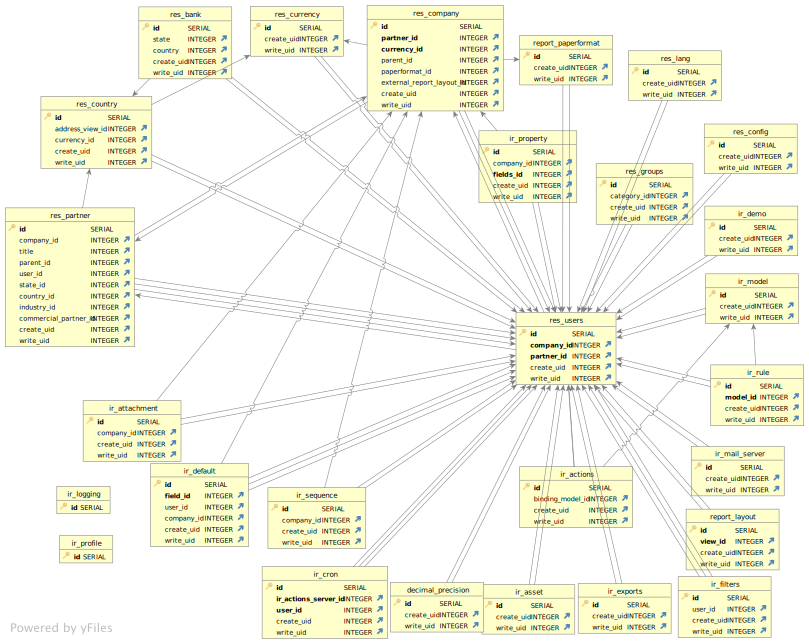
\includegraphics[width=14cm]{img/OdooCoreERD.png}
	\captionof{figure}{Skema Database Odoo }
	\label{fig:asd}
\end{center}



